%! Author = amatarazzo
%! Date = 06/04/24

\chapter{Foundations of Large Language Models}
\label{ch:foundations-of-large-language-models}

Large Language Models (LLMs) have revolutionized the field of Natural Language Processing (NLP) by achieving state-of-the-art performance on a wide range of tasks, such as text generation, text classification, and machine translation.\\
These models are trained on vast amounts of text data to learn the underlying structure of the language and capture the relationships between words.\\

In the following sections, we will explore the key concepts and techniques that underpin the development of LLMs, including pre-training strategies and major datasets used for training and evaluation, as well as the Transformer architecture, which forms the basis of many modern LLMs.\\

Finally, we will discuss some model adaptation techniques that can be used to fine-tune LLMs for specific tasks or domains.

\section{Pre-training strategies}
\label{sec:pre-training-strategies}

Pre-training constitutes a foundational phase in the development of Large Language Models (LLMs).
It allows the model to capture the relationships between words and generate coherent and contextually relevant text, laying the groundwork for its subsequent performance on specific NLP tasks~\cite{devlin2019bert, brown2020language}.\\
This phase involves training a language model on a vast corpus of text data before fine-tuning it on a smaller, task-specific dataset, such as text generation or text classification, to improve its performance on that task.\\
Moreover, the extensive pre-training on diverse corpora enables LLMs to develop a broad understanding, making them adaptable to a wide range of domains and languages~\cite{liu2019roberta, radford2019language}.

Despite its advantages, pre-training LLMs is not without its challenges.
The process requires substantial computational resources and energy, raising concerns about its environmental impact~\cite{strubell2019energy}.\\
Additionally, the data used for pre-training can influence the model's biases and sensitivities, necessitating careful curation of the training corpus to mitigate potential ethical and fairness issues~\cite{bender2021dangers}.\\
The field is evolving towards more efficient pre-training methods, such as transfer learning, where a pre-trained model is adapted to new tasks or languages with minimal additional training~\cite{ruder2019transfer}.\\
Moreover, emerging approaches aim to enhance the contextual awareness and ethical sensitivity of LLMs during the pre-training phase, addressing the challenges of bias and fairness head-on.\\

There are several pre-training strategies that have been used to train large language models, including unsupervised pre-training, supervised pre-training, and semi-supervised pre-training.
Let's explore each of these strategies in more detail.

\subsection{Unsupervised pre-training}
\label{subsec:unsupervised-pre-training}

Unsupervised pre-training is a pre-training strategy that involves training a model on a large corpus of text data without any labels or annotations.\\
The model is trained to predict the next word in a sequence of words, given the previous words in the sequence~\cite{brown2020language}.
This is done using a technique called Autoregressive Language Modeling (ALM), where the model is trained to predict the probability distribution over the next word in the sequence given the previous words in the sequence in a unidirectional manner.\\
Models like GPT-3 and its variants use this autoregressive language modeling objective to pre-train on large text corpora and learn the relationships between words in the language.\\
The main idea behind ALM is the prediction of the next token in a sequence based on the tokens that precede it.
The computational realization of this modeling approach is typically achieved through neural networks, particularly transformers, which leverage self-attention mechanisms to encapsulate dependencies across varying distances in the input sequence \cite{vaswani2023attention}.
During the generation process, a token is sampled based on the probability distribution predicted by the model for the next token position, appended to the sequence, and this augmented sequence is then fed back into the model iteratively to generate subsequent tokens~\cite{brown2020language}.
Despite its prowess, the autoregressive nature of these models imbues them with an intrinsic limitation: the inability to leverage future context in token prediction, constraining their context comprehension to a unidirectional scope.\\
BERT and its variants, on the other hand, employ a masked language model (MLM) objective, where random words in a sentence are masked, and the model is trained to predict these masked words based on their context, integrating both preceding and succeeding context in representation learning~\cite{devlin2019bert}.


\subsection{Supervised pre-training}
\label{subsec:supervised-pre-training}

Supervised pre-training is a pre-training strategy that involves training a model on a large corpus of text data with labels or annotations.
This paradigm contrasts with unsupervised pre-training, where models learn from raw text without explicit labels.
The supervised approach enables models to learn representations that are more closely aligned with the end tasks, potentially enhancing their performance and efficiency~\cite{gururangan2020don}.\\

\begin{figure}[H]
	\centering
	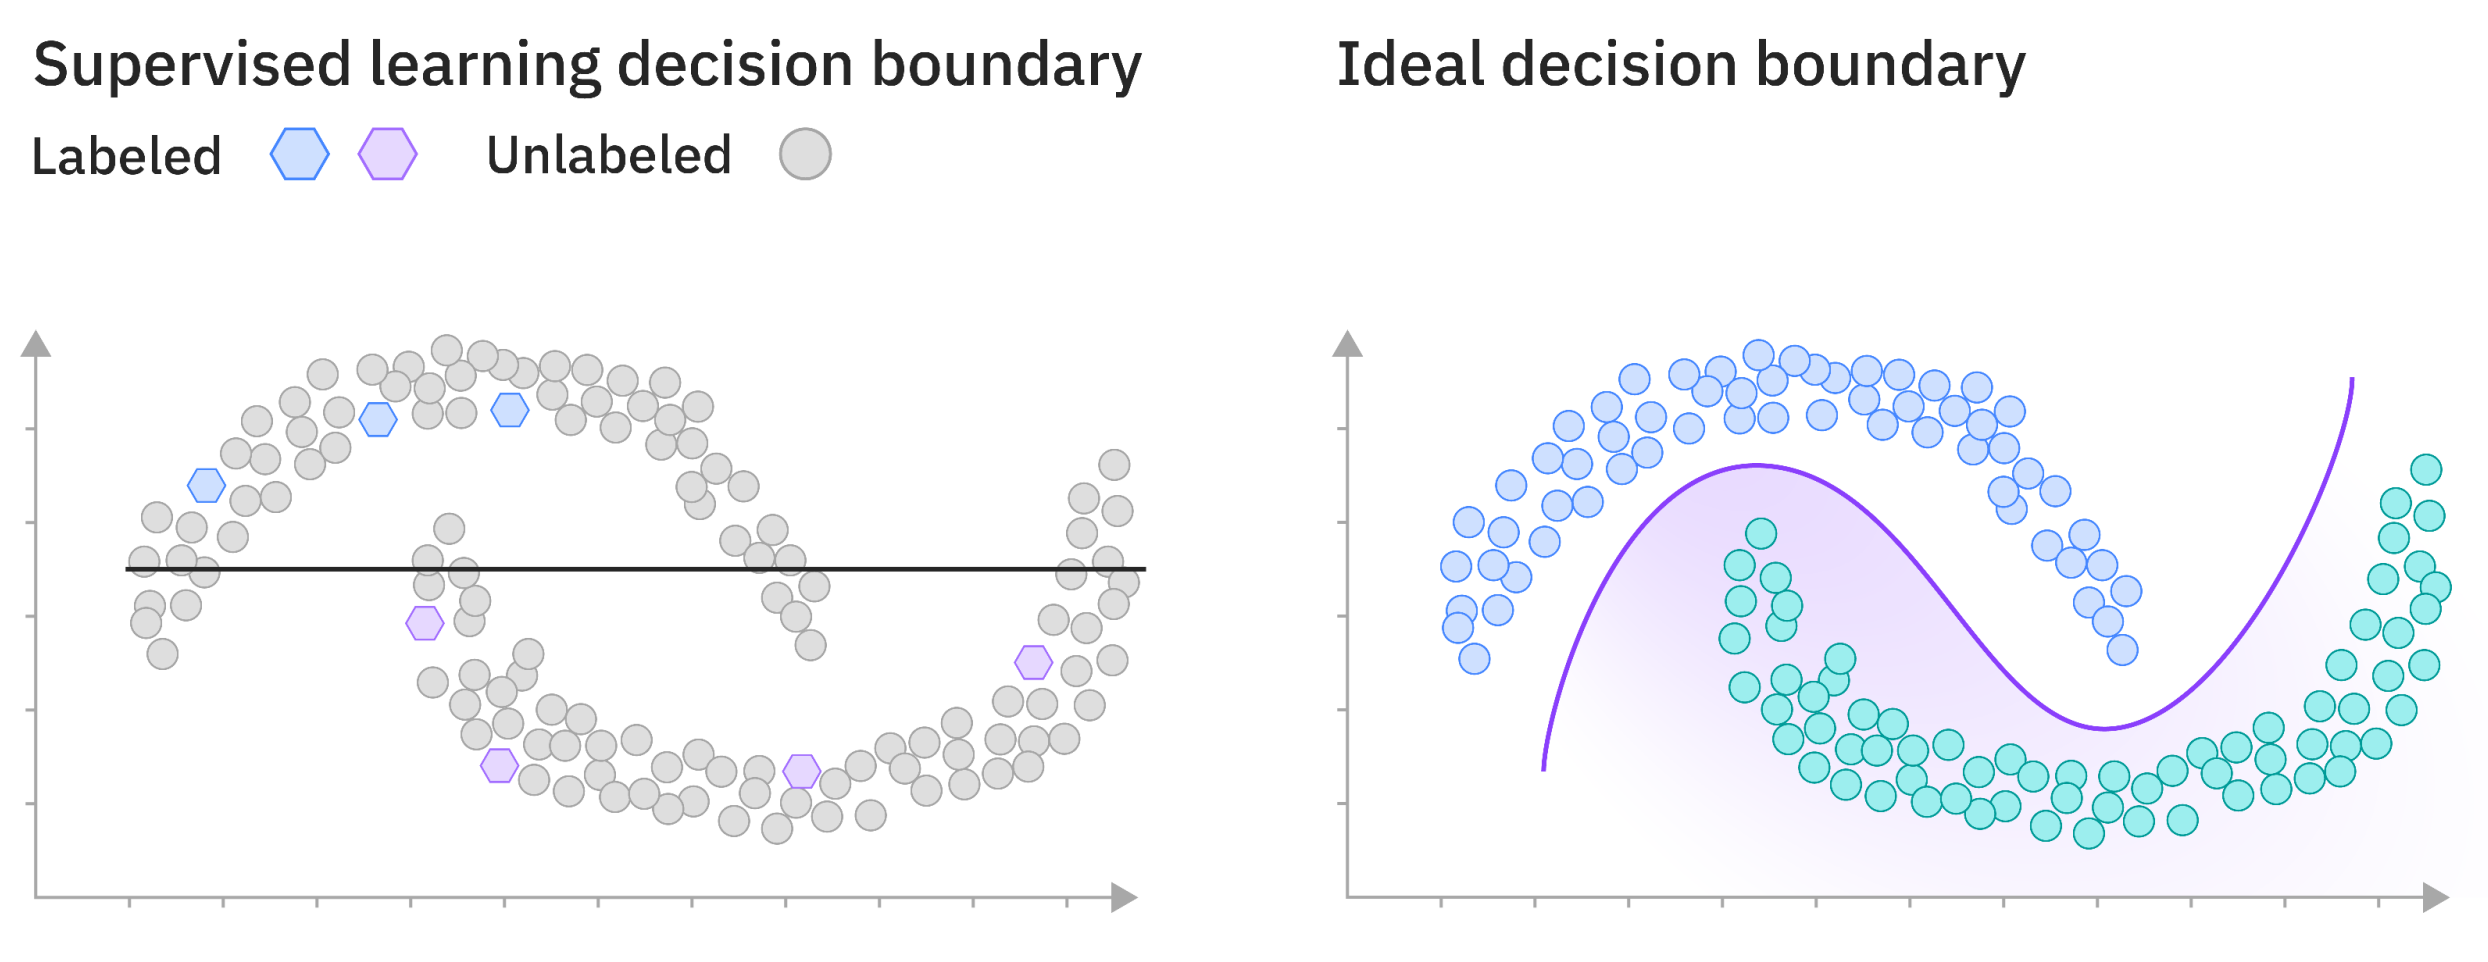
\includegraphics[width=\textwidth]{supervised}
	\caption{Using only the very limited labeled data points available, a supervised model may learn a decision boundary that will generalize poorly and be prone to misclassifying new examples. Source: \textcite{bergmann2023semi}.}
	\label{fig:supervised}
\end{figure}

In supervised pre-training, LLMs are exposed to a vast array of labeled data across various domains.
This training regime involves teaching the model to predict the correct output given an input, under the supervision of known input-output pairs.
This approach not only helps in learning general language representations but also imbues the model with domain-specific knowledge, which is particularly beneficial when the subsequent fine-tuning task is closely related to the pre-training data~\cite{phang2019sentence}.\\
One significant advantage of supervised pre-training is its potential to reduce the amount of labeled data required for fine-tuning on specific tasks.
By learning robust representations during pre-training, LLMs can achieve high performance on downstream tasks even with relatively smaller datasets, a concept known as transfer learning~\cite{ruder2019transfer}.
Moreover, supervised pre-training can lead to improvements in model generalization, making LLMs more adept at handling unseen data or tasks that diverge from their initial training corpus.\\

The reliance on large labeled datasets introduces concerns regarding the cost and feasibility of data annotation, especially in specialized domains where expert knowledge is required.\\
Furthermore, as shown in Figure~\ref{fig:supervised}, the risk of overfitting to the pre-training data is non-trivial, necessitating careful regularization and validation to ensure the model's generalizability~\cite{howard2018universal}.

\subsection{Semi-supervised pre-training}
\label{subsec:semi-supervised-pre-training}

Semi-supervised pre-training emerges as a compelling paradigm in the evolution of Large Language Models (LLMs), blending the strengths of supervised and unsupervised learning methodologies.
This hybrid training approach leverages a combination of labeled and unlabeled data, optimizing the utilization of available information and enhancing the model's learning efficacy and adaptability~\cite{zhu2005semi, chapelle2009semi}.\\

At its core, semi-supervised pre-training involves the initial training of models using a vast corpus of unlabeled data, akin to unsupervised pre-training.
This phase allows the model to capture a broad understanding of language structures and patterns.
Subsequently, the model undergoes further training or fine-tuning on a smaller labeled dataset, which instills task-specific knowledge and nuances \cite{ruder2019transfer, yang2017transfer}.\\
The rationale behind this approach is to exploit the abundance of readily available unlabeled data to develop a comprehensive language model, which is then refined using the more scarce labeled data to achieve superior performance on target tasks.\\

Various techniques underpin semi-supervised pre-training in LLMs.
One prominent method involves self-training, where the model, initially trained on labeled data, generates pseudo-labels for the unlabeled dataset.
These pseudo-labeled data points are then incorporated into further training cycles, iteratively enhancing the model's accuracy and robustness~\cite{lee2013pseudo}.
Another notable technique is the use of consistency regularization, which ensures that the model produces similar outputs for perturbed versions of the same input data, enhancing the model's stability and generalization capabilities~\cite{sajjadi2016regularization}.
Other Key techniques in semi-supervised learning include transductive and inductive learning, with practical methods like label propagation and active learning aiding in leveraging unlabeled data.
These approaches are instrumental in refining the model's decision-making capabilities~\cite{bergmann2023semi}.\\
Transductive learning, a concept primarily attributed to \textcite{vapnik1998statistical}, focuses on predicting specific examples from the training set without attempting to generalize beyond those.
In transductive inference, the model is directly applied to the specific test set, aiming to infer the correct labels for the given unlabeled data.
The key characteristic distinguishing transductive learning from other machine learning methods is its focus on the particular sample at hand rather than on a general rule applicable to new, unseen instances.\\
One of the main applications of transductive learning is in the realm of support vector machines (SVMs), where it is employed to predict labels for a given, fixed set of test data, optimizing the margin not only for the training data but also for the test data, despite their labels being unknown~\cite{joachims1999transductive}.\\

Conversely, inductive learning aims to build a general model that predicts outcomes for new, unseen data based on the patterns learned from the training data.
Label propagation (Figure~\ref{fig:label_propagation}) is a common technique in inductive learning, where the model infers the labels of unlabeled data points based on the labels of their neighbors in the feature space.

\begin{figure}[H]
	\centering
	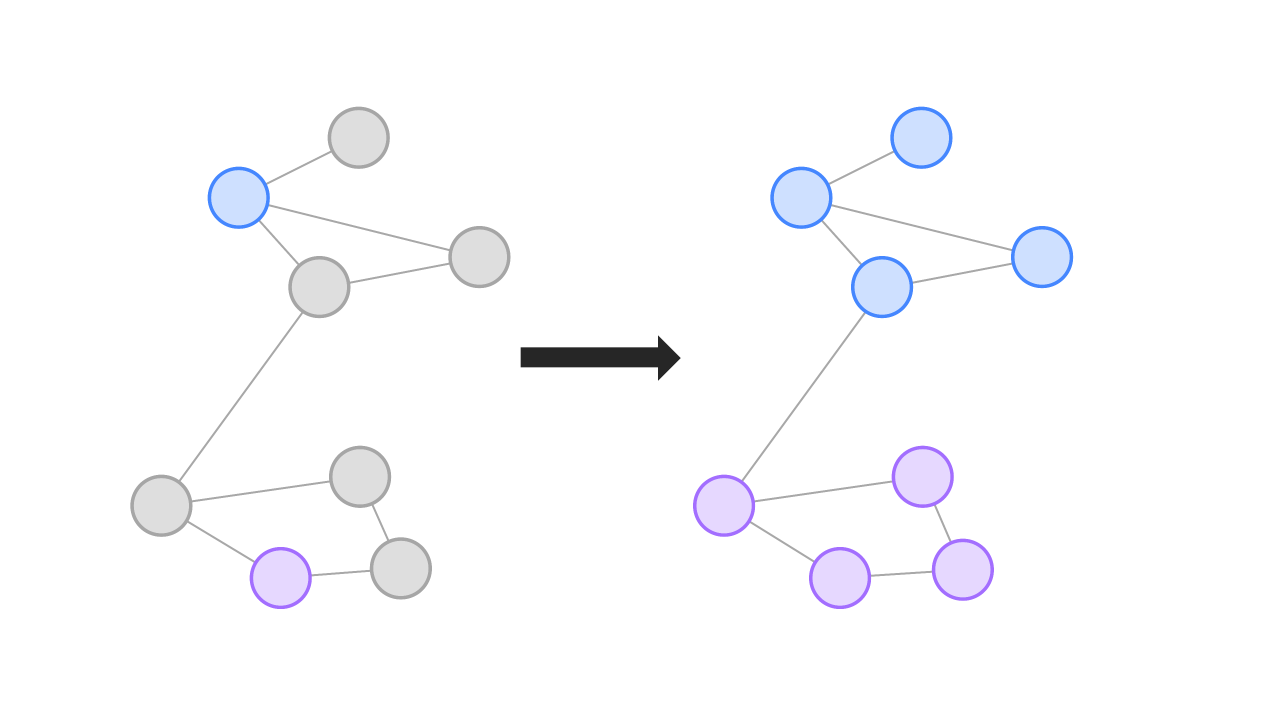
\includegraphics[width=\textwidth]{label_propagation}
	\caption{LEFT: original labeled and unlabeled data points. RIGHT: using label propagation, the unlabeled data points have been assigned pseudo-labels. Source: \textcite{bergmann2023semi}.}
	\label{fig:label_propagation}
\end{figure}

Active learning is another inductive learning method that involves iteratively selecting the most informative data points for labeling, optimizing the model's performance with minimal labeled data.\\
This approach is more general than transductive learning and underpins most supervised learning algorithms.
The objective here is to infer a function that can generalize well across unseen samples, not just the examples provided during the training phase.\\
Inductive learning is fundamental to numerous machine learning algorithms, from linear regression to deep neural networks, where the model learns an underlying function that maps input data to output predictions, with the hope that this function will perform accurately on data not present in the training set~\cite{mitchell1997machine}.\\

Semi-supervised approach is predicated on certain assumptions about the underlying structure and distribution of the data, which facilitate the effective integration of unlabeled data into the learning process.
\begin{itemize}
	\item \textbf{Cluster Assumption:} {The cluster assumption posits that data points within the same cluster are more likely to share a label. This assumption underpins the idea that data points in high-density regions of the input space belong to the same class, while low-density regions denote boundaries between classes~\cite{chapelle2009semi}. This principle guides the model to generalize from labeled data points to nearby unlabeled ones within the same cluster.}
	\item \textbf{Continuity Assumption:} {Also known as the smoothness assumption, this posits that if two points in the input space are close to each other, than their corresponding outputs are also likely to be similar~\cite{zhou2004learning}. In practical terms, this means that if two data points are close in the feature space, they are likely to share the same label.}
	\item \textbf{Manifold Assumption:} {The manifold assumption suggests that high-dimensional data lie on a low-dimensional manifold. This assumption implies that the data points are situated on a manifold of much lower dimensionality embedded within the higher-dimensional space, and learning can be simplified if this manifold structure is discovered and exploited~\cite{belkin2006manifold}. The manifold assumption often complements the cluster and continuity assumptions, providing a geometric interpretation of the data's distribution.}
	\item \textbf{Low-Density Separation Assumption:} {This assumption posits that the decision boundary between different classes should lie in regions of low data density~\cite{chapelle2009semi}. Essentially, it is expected that there is a natural separation or gap between classes, and the learning algorithm should prefer hypotheses that place the decision boundary in regions where few data points are present.}
\end{itemize}

\section{Commonly-used data sources}
\label{sec:commonly-used-data-sources}

The development and evaluation of Large Language Models (LLMs) rely heavily on the availability of high-quality datasets that span diverse domains and languages.
The datasets in Table~\ref{tab:table} serve as the foundation for pre-training and fine-tuning LLMs, enabling researchers to assess the models' performance on a wide range of tasks, from text generation to machine translation.\\

\begin{table}[H]
	\centering
	\begin{tabularx}{\textwidth}{|X|X|X|X|}
		\hline
		\textbf{Corpora}                           & \textbf{Size} & \textbf{Source} & \textbf{Latest Update Time} \\
		\hline
		BookCorpus~\cite{zhu2015aligning}          & 5GB           & Books           & Dec-2015                    \\
		Gutenberg~\cite{projectgutenberg}          & -             & Books           & Dec-2021                    \\
		C4~\cite{t5}                               & 800GB         & CommonCrawl     & Apr-2019                    \\
		CC-Stories-R~\cite{trinh2018simple}        & 31GB          & CommonCrawl     & Sep-2019                    \\
		CC-NEWS~\cite{liu2019roberta}              & 78GB          & CommonCrawl     & Feb-2019                    \\
		REALNEWS~\cite{zellers2019defending}       & 120GB         & CommonCrawl     & Apr-2019                    \\
		OpenWebText~\cite{gokaslan2019openwebtext} & 38GB          & Reddit links    & Mar-2023                    \\
		Pushift.io~\cite{baumgartner2020pushshift} & 2TB           & Reddit links    & Mar-2023                    \\
		Wikipedia~\cite{wikipedia}                 & 21GB          & Wikipedia       & Mar-2023                    \\
		BigQuery~\cite{bigquerydataset}            & -             & Codes           & Dec-2023                    \\
		the Pile~\cite{gao2021pile}                & 800GB         & Other           & Dec-2020                    \\
		ROOTS~\cite{laurencon2022bigscience}       & 1.6TB         & Other           & Jun-2022                    \\
		\hline
	\end{tabularx}
	\caption{Statistics of commonly-used data sources. Source: \textcite{survey}}
	\label{tab:table}
\end{table}

In this section, we will explore some of the most commonly-used data sources for training and evaluating LLMs.
Based on their content types, we catego- rize these corpora into six groups: Books, CommonCrawl, Reddit links, Wikipedia, Code, and others.

\begin{itemize}
	\item \textbf{Books:} {
		      BookCorpus~\cite{zhu2015aligning} and Gutenberg~\cite{projectgutenberg} are two prominent datasets that contain text from a wide range of books, spanning various genres and topics. These datasets are valuable for training LLMs on literary text and assessing their performance on text generation tasks.\\
		      BookCorpus is a dataset consisting of text from over 11,000 books (e.g., novels and biographies), while Gutenberg is a collection of over 70,000 free ebooks including novels, essays, poetry, drama, history, science, philosophy, and other types of works in the public domain -- used for training of LLaMa~\cite{touvron2023llama}.
	      }
	\item \textbf{CommonCrawl:} {
		      CommonCrawl~\cite{commoncrawl} is a vast web corpus that contains data from billions of web pages, covering diverse topics and languages. Due to noise and redundancy in the data, researchers often extract subsets of CommonCrawl for training LLMs. The main subsets used for training LLMs are C4\footnote{Colossal Clean Crawled Corpus}~\cite{t5}, CC-Stories-R~\cite{trinh2018simple}, CC-NEWS~\cite{liu2019roberta}, and REALNEWS~\cite{zellers2019defending}.\\
	      }
	\item \textbf{Reddit links:} {
		      Reddit is a social media platform where users can submit links and posts and "upvotes" or "downvote" them. Posts with high number of "upvotes" are often considered useful, and can be used to create high-quality datasets.
		      OpenWebText~\cite{gokaslan2019openwebtext} and Pushshift.io~\cite{baumgartner2020pushshift} are datasets that contain text data extracted from Reddit. These datasets are useful for training LLMs on social media text and assessing their performance on text generation and sentiment analysis tasks.
	      }
	\item \textbf{Wikipedia:} {
		      Wikipedia~\cite{wikipedia} is a widely-used dataset that contains text from articles on various topics. It's an online encyclopedia with a large volume of high-quality articles. Most of these articles are composed in an expository style of writing (with supporting references), covering a wide range of languages and fields.
		      Typically, the English-only filtered versions of Wikipedia are widely used in most LLMs (e.g., GPT-3~\cite{brown2020language}, and LLaMA~\cite{touvron2023llama}).
		      Wikipedia is available in multiple languages, so it can be used in multilingual settings.
	      }
	\item \textbf{Code:} {
		      Two major sources are GitHub for open-source licenses and StackOverflow for code-related question-answering platforms.\\
		      Google has publicly released the BigQuery, a dataset that contains code snippets from various programming languages. This dataset is useful for training LLMs (i.e., CodeGen) on code text and assessing their performance on code generation and code completion tasks.
	      }
	\item \textbf{Others:} {
		      The Pile and ROOTS are datasets that contain text data from various sources, such as books, articles, and websites.\\
		      The Pile contains 800GB of data from multiple sources, including books, websites, codes, scientific papers, and social media platforms.\\
		      ROOTS is composed of various smaller datasets (totally 1.61 TB of text) and covers 59 different languages (containing natural languages and programming languages).
	      }
\end{itemize}